\documentclass[11pt,letterpaper]{article}
\usepackage[margin=1in,headheight=14pt]{geometry}
\usepackage[T1]{fontenc}
\usepackage[utf8]{inputenc}
\usepackage{amsmath,amsthm}
\usepackage{newtxtext,newtxmath}
\usepackage{microtype}
\usepackage{graphicx,booktabs,tabularx,array,multirow}
\usepackage{caption}
\usepackage{enumitem}
\usepackage{setspace}
\usepackage[round,authoryear]{natbib}
% Deliberate departure from the template this paper's formatting follows. The
% template leaves the author-year separator empty, giving "(MSCI Inc. 2012)".
% APA requires a comma there, so the fifth argument is set rather than left
% blank. Every other punctuation choice is the template's.
\bibpunct{(}{)}{,}{a}{,}{,}

\providecommand{\SohamLocation}{\textit{India}}

\usepackage{xurl}
\usepackage[hidelinks]{hyperref}
\usepackage{fancyhdr}
\usepackage{placeins}
\usepackage{etoolbox}
\hypersetup{%
  pdftitle={Replicating USMV and SPLV with a Public-Data Factor Risk Model},
  pdfauthor={Soham Abhay Parundekar},
  pdfsubject={Specification ambiguity dominates the choice of covariance
              estimator},
  pdfkeywords={minimum volatility, index replication, factor risk model,
               covariance estimation, portfolio constraints}}
\setstretch{1.06}
\setlength{\parindent}{1em}
\setlength{\parskip}{3pt}
\setlength{\emergencystretch}{2em}
\clubpenalty=10000
\widowpenalty=10000
\setlength{\textfloatsep}{13pt plus 3pt minus 3pt}
\setlength{\floatsep}{11pt plus 2pt minus 2pt}
\captionsetup{font=small,labelfont=bf,labelsep=period,justification=raggedright,singlelinecheck=false,skip=7pt}
\setcounter{topnumber}{2}
\setcounter{totalnumber}{3}
\renewcommand{\topfraction}{0.90}
\renewcommand{\textfraction}{0.08}
\renewcommand{\floatpagefraction}{0.80}
\pagestyle{fancy}
\fancyhf{}
\fancyhead[L]{\footnotesize Replicating USMV and SPLV}
\fancyfoot[C]{\thepage}
\renewcommand{\headrulewidth}{0.25pt}
\newcolumntype{Y}{>{\raggedright\arraybackslash}X}
\newcommand{\E}{\mathbb{E}}
\newcommand{\Var}{\operatorname{Var}}
\newcommand{\diag}{\operatorname{diag}}
\newcommand{\sgn}{\operatorname{sgn}}
\newcommand{\ind}{\mathbf{1}}
\newcommand{\F}{\mathcal{F}}
\newcommand{\notetext}[1]{\vspace{4pt}\par\noindent{\footnotesize\raggedright #1\par}}
\newtheorem{proposition}{Proposition}
\newtheorem{remark}{Remark}
\renewcommand{\arraystretch}{1.12}

% Shorthands for the objects compared throughout. Defined once so a change of
% notation cannot drift between sections.
\newcommand{\wvec}{w}                  % optimised index weights
\newcommand{\bvec}{b}                  % parent index weights
\newcommand{\Sig}{\Sigma}              % asset covariance
\newcommand{\Xsty}{X^{\mathrm{sty}}}   % standardised style exposures
\newcommand{\Xind}{X^{\mathrm{ind}}}   % industry membership dummies

\begin{document}

\thispagestyle{plain}
\begin{center}
{\LARGE\bfseries Replicating USMV and SPLV with a public-data factor risk
model\par}
\vspace{7pt}
{\large Specification ambiguity dominates the choice of covariance
estimator\par}
\vspace{14pt}

\begingroup
\setlength{\tabcolsep}{5pt}
\renewcommand{\arraystretch}{1.0}
\newcommand{\AuthorBlock}[3]{%
  {\fontsize{10.1}{11.7}\selectfont\bfseries #1\par}%
  \vspace{1.5pt}%
  {\fontsize{8.0}{9.4}\selectfont\href{mailto:#2}{\nolinkurl{#2}}\par}%
  \vspace{1.0pt}%
  {\fontsize{8.5}{10.0}\selectfont Independent Researcher, #3\par}%
}
\AuthorBlock{Soham Abhay Parundekar}{parundekarsoham@gmail.com}{\SohamLocation}
\endgroup
\end{center}

% Abstract. Every number carries a ledger id: TE figures E01a/E02a/E03a, the
% difference E04, the estimator spread E10, the BAB range E18, active sector
% E19a/E19b. Precision follows the ledger and must not be adjusted here.
\begin{abstract}
A published index methodology is not a complete specification. We rebuild two
low-volatility equity indices from free public data, one defined by a
constrained optimiser over a commercial factor risk model and one by a rank and
inverse-volatility rule, and ask how much of each is recoverable. The
transparent rule is almost fully recoverable: it tracks its fund at 1.62\%
annualised tracking error with a correlation of 0.9939. The optimiser is not,
at 5.83\%. The residual is not covariance estimation. Four estimators spanning
a sample matrix, a two-half-life structural model, constant-correlation
shrinkage and a Bai--Ng-selected principal-component model produce realised
volatilities 25 basis points apart under an identical constraint set, which is
what prior work reports for constrained portfolios generally. Resolving one
ambiguity in the published constraint document moves tracking error by 2.10
percentage points. The methodology exempts a single proprietary volatility
factor from its style bands; a replicator with a different factor set must
decide whether that exemption covers residual volatility alone or beta as well,
and exempting both brings tracking error to 3.73\%, replica volatility to
13.97\% against the fund's 13.45\%, and the beta to the fund to 1.001. On this
evidence the specification choice is worth roughly an order of magnitude more
than the estimator choice, for this index pair over this sample; we do not
establish that ordering in general. What the constraints deliver is control
rather than lower realised risk, holding the largest active industry weight
near its five per cent band where the heuristic averages 40.7\%. No portfolio
shows a six-factor alpha significant at the five per cent level, and
betting-against-beta loadings between 8.7 and 14.0 absorb what intercept there
is.
\end{abstract}
\noindent\textit{Keywords:} minimum volatility; index replication; factor risk model; covariance estimation; portfolio constraints.\par
\noindent\textit{JEL classification:} C13, C58, G11, G12, G17.
\vspace{8pt}


\section{Introduction}
\label{sec:intro}
Two of the largest low-volatility equity funds are built on opposite
philosophies. The iShares MSCI USA Min Vol Factor ETF, USMV, tracks an index
defined by a constrained quadratic programme over a commercial multi-factor
risk model \citep{ishares2011usmv497k}. The Invesco S\&P 500 Low Volatility
ETF, SPLV, tracks an index defined by two sentences: take the hundred least
volatile members of the parent, weight them by the inverse of their volatility
\citep{invesco2024splv497k}. Both providers publish their rules. Only one of
them publishes rules a reader can act on.

That asymmetry is the subject of this paper. A rank-and-weight rule is complete
in the sense that two people implementing it from the document will produce the
same portfolio. A constrained optimisation is not, because the constraints are
written in the vocabulary of the provider's own risk model. The weight cap,
the sector band and the turnover limit survive translation. The style-factor
band does not: it is stated relative to standardised exposures to factors the
provider names but does not define, and a replicator with a different factor
set has to decide what those names map onto. The decision is invisible in the
methodology document and consequential in the result.

This is a different problem from index tracking as that literature usually
poses it. There the index is taken as given and the task is to approximate its
return series with a manageable subset of its constituents, whether by
optimisation, by statistical factorisation or by learned models; recent
treatments include \citet{cesarone2025benchmark}, and \citet{dhingra2026index}
survey the field. We are not approximating a return series. We are
reconstructing the rule that generates it, from the document that states the
rule, and asking what that document leaves undetermined. Tracking error appears
here as the measure of how well the reconstruction succeeded, not as an
objective anything was optimised against.

We quantify how consequential. Using a weekly factor risk model built entirely
from free data, we rebuild both indices over the funds' own lifetimes and
measure each replica against the fund that tracks the index it targets. The
SPLV replica achieves 1.62\% annualised tracking error with a correlation of
0.9939, close enough that the remaining difference is mostly the
parent-universe proxy. The USMV replica achieves 5.83\%. Closing that gap is
where the paper's content lies, and the usual suspect turns out to be the wrong
one.

The usual suspect is the covariance matrix. If a commercial risk model is the
thing a free-data replication cannot reproduce, then a better covariance
estimate should narrow the gap, and the literature offers a well-stocked menu
of them. We run four: the sample matrix, a two-half-life structural factor
model in the Barra idiom, constant-correlation shrinkage after
\citet{ledoit2003improved}, and a principal-component model whose factor count
is chosen by the \citet{bai2002determining} criteria rather than assumed. Under
one specification they track the fund within 26 basis points of one another. That is the ordering \citet{dom2025beyond} report for constrained
portfolios in general, and \citet{jagannathan2003risk} supply the reason:
binding weight constraints act as a form of shrinkage, so a portfolio that is
already constrained has less to gain from a better estimate of $\Sig$. Our
contribution on this point is a confirmation in a specific published
constraint set, not a new result.

The specification choice is worth far more. The methodology exempts one
proprietary volatility factor from the style bands, which is the entire
mechanism by which a minimum-volatility index is permitted to be a
low-volatility index. A public-data model has two candidates for what that
factor names, beta and residual volatility, and the document that governs the
index in question does not say which. Exempting residual volatility alone gives
5.83\%. Exempting beta as well gives 3.73\%, with replica volatility of 13.97\%
against the fund's 13.45\% and a beta to the fund of 1.001. One sentence in a
constraint document, read two defensible ways, moves tracking error by 2.10
percentage points, eight times what the choice among four covariance estimators
moves the same quantity. The two are not close: a circular block bootstrap on
daily active returns puts the exemption effect at [1.84, 2.35] percentage
points and the estimator spread at [0.15, 0.40], and the first exceeds the
second in all 2{,}000 resamples.

We also report what the constraints buy, since the comparison invites the
question of whether the optimiser earns its complexity. On realised volatility
it does not: over this sample the optimised replicas are more volatile than the
heuristic one, not less. What the constraints deliver is control over where the
risk sits. The sector band binds at every review we examine, holding the
largest active industry weight at five per cent, while the unconstrained rule
drifts to between 32 and 48 per cent, growing monotonically across its reviews
as a single industry became both larger in the parent and more volatile. The
two sets of review dates do not coincide, so this is a contrast between a
binding constraint and its absence rather than a matched comparison; it is also
not a close call. Neither index produces a six-factor alpha significant
at the five per cent level, and betting-against-beta loadings between 8.7 and
14.0 absorb what intercept there is, which is consistent with the
leverage-constraint account of \citet{frazzini2014betting} and does not
distinguish it from the benchmarking account of \citet{baker2011benchmarks}.

Three boundaries on all of this. The parent universe is a proxy: the optimiser
works over the S\&P 500 where the real index uses a broader one, and that
substitution is the largest single contributor to the optimised tracking error
and cannot be repaired by anything else in the pipeline. The ordering between
specification and estimation is measured on one index pair over one sample
period, so it is a demonstration that the ordering can be this large, not a
claim that it is this large in general. And the minimum-holding rule makes the
programme mixed-integer; we handle it with the drop-and-resolve heuristic that
index providers themselves describe, and we do not measure the gap to an exact
solve. Section~\ref{sec:limits} sets these out in full.

Section~\ref{sec:rules} states both index rules from their primary documents and
identifies precisely what the optimised one leaves open.
Section~\ref{sec:model} builds the risk model and Section~\ref{sec:data} the
data behind it, including the three ways free price and fundamental data will
mislead a replication that does not defend against them.
Section~\ref{sec:design} gives the replication design.
Sections~\ref{sec:repro} to \ref{sec:anomaly} report what is reproducible,
whether the estimator matters, what the constraints buy, and whether any of it
is an anomaly. Section~\ref{sec:limits} and Section~\ref{sec:conclusion}
interpret and conclude.

\section{The two index rules, and what the documents do not settle}
\label{sec:rules}

\subsection{The optimised rule}
The minimum-volatility index is the solution to a quadratic programme. With
$\wvec$ the index weights, $\bvec$ the parent index weights, $\Sig$ the
provider's estimated asset covariance matrix, $S$ a sector-membership matrix
and $\Xsty$ the standardised style exposures, the published constraint set is

\begin{align}
 \min_{\wvec}\ & \wvec^{\top}\Sig\wvec \label{eq:qp}\\
 \text{s.t.}\ & \ind^{\top}\wvec = 1, \nonumber\\
 & 0 \le \wvec_i \le \min(1.5\%,\ 20\,\bvec_i) \quad \forall i, \nonumber\\
 & \wvec_i = 0 \ \text{ or } \ \wvec_i \ge 0.05\% \quad \forall i, \nonumber\\
 & \bigl|S^{\top}(\wvec-\bvec)\bigr| \le 5\% \quad \text{per sector},
   \nonumber\\
 & \bigl|\Xsty_{-v}{}^{\!\top}(\wvec-\bvec)\bigr| \le 0.25 \quad
   \text{per non-exempt style}, \nonumber\\
 & \tfrac{1}{2}\lVert \wvec-\wvec_{\rm prev}\rVert_1 \le 10\%. \nonumber
\end{align}

The index is reviewed semi-annually, effective the last business day of May and
November, and the covariance matrix is dated to the end of the month preceding
the review rather than to the review itself \citep{msci2012minvol}. Where the
constraint set admits no feasible point the methodology prescribes a relaxation
sequence, loosening turnover first, then the minimum holding, then the weight
cap and sector band together, and never the style bands; Appendix~\ref{app:ladder}
gives the sequence as implemented.

Three features of \eqref{eq:qp} deserve note before the replication. The
semi-continuous condition on $\wvec_i$ makes the programme mixed-integer: a
holding is either absent or at least five basis points, with nothing in
between, which rules out the continuum of dust positions a plain quadratic
programme would return. The turnover constraint is written against
$\wvec_{\rm prev}$, which is the previous book after it has drifted with
prices, not the previous optimisation target. And $\Xsty_{-v}$ carries a
subscript doing a great deal of work: it is the style block with the volatility
factor removed, and that removal is the whole mechanism by which the programme
is allowed to produce a low-volatility portfolio rather than merely a
constrained one.

\subsection{The heuristic rule}
The low-volatility index is specified in two sentences. From the parent
constituents, select the hundred securities with the lowest realised volatility
over the trailing year of trading days; weight each in proportion to the
reciprocal of that volatility, normalised to sum to one
\citep{invesco2024splv497k}. Formally, with $\sigma_i$ the trailing volatility
and $\mathcal{L}$ the hundred lowest,

\begin{equation}
 \wvec_i = \frac{\sigma_i^{-1}}{\sum_{j\in\mathcal{L}}\sigma_j^{-1}}
 \quad \text{for } i\in\mathcal{L}, \qquad \wvec_i = 0 \text{ otherwise.}
 \label{eq:splv}
\end{equation}

There is no covariance matrix, no sector constraint, no style constraint and no
turnover limit. Rebalancing is quarterly. The rule uses only the diagonal of
the covariance matrix, and only its square root at that.

% Table 1. Descriptive, not empirical: every cell is a provision read off the
% primary documents cited in the note, so there is no frozen output behind it
% and make_tables.py does not generate it. Values must be changed only against
% the source documents.
\begin{table}[tbp]
\caption{The two published rules, side by side.}
\label{tab:rules}
\centering\small
\setlength{\tabcolsep}{5pt}
\begin{tabularx}{\textwidth}{@{}lYY@{}}
\toprule
 & Optimised index & Heuristic index\\
\midrule
Objective        & Minimise predicted variance & None stated\\
Risk input       & Full covariance matrix from a commercial factor model
                 & Trailing one-year realised volatility, per stock\\
Selection        & Implied by the programme & The 100 lowest-volatility
                   parent members\\
Weighting        & Implied by the programme & Proportional to
                   $1/\sigma_i$\\
\addlinespace
Weight cap       & $\min(1.5\%,\ 20\times$ parent weight$)$ & None\\
Minimum holding  & 0.05\%, or zero & None\\
Sector band      & $\pm5\%$ active per sector & None\\
Style band       & $\pm0.25$ SD active per style, volatility exempt & None\\
Turnover cap     & 10\% one-way per review & None\\
\addlinespace
Review frequency & Semi-annual & Quarterly\\
Effective date   & Last business day of May and November
                 & Third Friday of the review month\\
Risk-model date  & End of the month preceding the review & Not applicable\\
Infeasibility    & Documented relaxation sequence & Cannot arise\\
\bottomrule
\end{tabularx}
\notetext{Provisions for the optimised index are from its provider's published
methodology \citep{msci2012minvol}; those for the heuristic index are from the
tracking fund's summary prospectus \citep{invesco2024splv497k}, which states the
selection and weighting rules in the issuer's own words. The heuristic index's
review calendar and effective date are the one entry in this table taken from
published convention rather than from a methodology document: the provider's
methodology PDF refused the request from the run environment and was not
retrieved, which Section~\ref{sec:limits} records as an unverified parameter.
The style band is the row that does not survive translation into another risk
model, and Section~\ref{sec:rules} takes it up.}
\end{table}


\subsection{What the style band does not settle}
Every constraint in \eqref{eq:qp} except one translates without ambiguity into
a replicator's own model. A 1.5\% cap is a 1.5\% cap. The sector band needs a
sector classification, and using a coarser one than the provider is a
documented approximation with a known direction of error. The turnover cap and
the minimum holding are numbers.

The style band is different in kind. It is stated in units of standardised
exposure to factors the methodology names but does not define, and the name it
gives the exempt factor is the name of a component of a proprietary model. The
document governing the index examined here exempts \emph{the Barra Volatility
risk index factor}, in the singular. A public-data factor model built to the
conventional recipe has two descriptors with an equally good claim to that
name: the beta of a stock's returns to the parent index, and the volatility of
the residual from that same regression. The first is systematic risk, the
second is the part orthogonal to it. Both are volatility in any ordinary sense,
and the published text does not choose between them.

The choice is not resolved by looking elsewhere in the provider's
documentation, though it is tempting to try. A later methodology covering the
provider's \emph{advanced} minimum-volatility family does enumerate the
exemption as two named factors, beta and residual volatility
\citep{msci2025minvoladvanced}. That document governs a different index family
from the one tracked here, so it cannot be read as a statement about this
index's constraint set. It establishes that the provider's own vocabulary
admits both readings, which is the opposite of settling the question.

A replicator therefore faces a genuine fork, and both branches are defensible.
Exempting residual volatility alone is the literal reading: one named factor,
one exemption, and residual volatility is the descriptor a risk model would
most naturally call volatility once beta has been accounted for separately.
Exempting beta as well is the functional reading: the purpose of the exemption
is to let the optimiser reduce risk, the optimiser's principal lever for
reducing risk is to hold low-beta stocks, and a $\pm0.25$ standard deviation
band on beta forecloses most of that lever before the programme starts.

We implement both and report both. Section~\ref{sec:repro} shows that the fork
is worth 2.10 percentage points of tracking error, and
Section~\ref{sec:estimator} that the choice among four covariance estimators is
worth a fortieth of that. The point is not that one reading is correct. It is
that a reader of the methodology document cannot tell which the index uses, and
that this single unresolved sentence dominates every estimation decision made
downstream of it.

\section{A factor risk model from public data}
\label{sec:model}
Replicating \eqref{eq:qp} requires a $\Sig$. This section builds one in the
conventional multi-factor idiom, from descriptors a reader can compute from
free sources, and then builds three alternatives to it so that
Section~\ref{sec:estimator} can ask whether the choice matters. Everything is
weekly: exposures are measured on Fridays, factor returns span Friday to
Friday, and the last available trading day substitutes when a Friday is a
holiday.

\subsection{Exposures}
Six style descriptors are computed for every name in the weekly cross-section:
the logarithm of market capitalisation; the beta of daily excess returns to the
cap-weighted parent over a trailing 252 days, shrunk toward one; the standard
deviation of the residual from that same regression; the cumulative return over
252 days skipping the most recent 21, which is the usual construction that
avoids one-month reversal; book equity over market capitalisation, with book
equity taken point-in-time as Section~\ref{sec:data} describes; and the
logarithm of average daily dollar volume over a trailing 63 days.

Beta is shrunk following \citet{blume1971assessment},
\begin{equation}
 \hat\beta_i^{\,\rm shrunk} = 0.67\,\hat\beta_i^{\,\rm raw} + 0.33,
 \label{eq:blume}
\end{equation}
with coefficients summing to one so the parent portfolio retains a beta of one.
The two-thirds weighting is a conventional choice rather than a value estimated
on this sample, and nothing in the results turns on the exact split.

Each raw descriptor is winsorised at its 1st and 99th cross-sectional
percentiles and then standardised twice over, to a capitalisation-weighted mean
of zero and an equal-weighted standard deviation of one:
\begin{equation}
 X_{ik} = \frac{d_{ik} - \sum_j b_j d_{jk}}
               {\operatorname{sd}_{\rm ew}\!\left(d_{\cdot k} -
                \textstyle\sum_j b_j d_{jk}\right)}.
 \label{eq:standardise}
\end{equation}
The asymmetry is deliberate and it is not cosmetic. Centring on the
cap-weighted mean makes the parent index's exposure exactly zero on every
style, which is what allows the $\pm0.25$ band in \eqref{eq:qp} to be read as a
deviation from the parent rather than from an arbitrary origin. Scaling by the
equal-weighted standard deviation keeps the unit of that band from being
dictated by the largest few names. A band stated in standard deviations is only
as meaningful as the standardisation underneath it, so a replication that
standardises differently from the provider is applying a different constraint
while appearing to apply the same one.

Standardisation uses only the names in that week's cross-section. Standardising
across the pooled history would let later information set the scale for earlier
weeks, which is look-ahead through a side door.

\subsection{Factor returns and an identification problem}
Weekly factor returns come from a cross-sectional regression of returns on the
exposures known at the start of the week,
\begin{equation}
 r_{i,t} = f^{\rm mkt}_t
         + \sum_j \Xind_{ij,t-1} f^{\rm ind}_{j,t}
         + \sum_k \Xsty_{ik,t-1} f^{\rm sty}_{k,t}
         + u_{i,t},
 \label{eq:csreg}
\end{equation}
fitted by weighted least squares with weights proportional to $\sqrt{b_i}$. The
square root is the Barra convention and sits between two bad alternatives: a
cap-weighted fit is effectively a regression on thirty mega caps, an
equal-weighted fit hands the estimate to the noisiest small names. Exposures
are dated $t-1$ and returns span $t-1$ to $t$. Several descriptors are built
from trailing returns, so fitting contemporaneous exposures would let the
regression explain part of the return with itself.

Equation~\eqref{eq:csreg} is rank deficient as written. Industry membership is
exhaustive and exclusive, so the industry dummies sum to the intercept for
every row and the market factor is not separately identified. The textbook
remedy is to drop one industry column, and it works numerically while quietly
changing what every coefficient means: the intercept stops being the market
return and becomes the omitted industry's return, and each remaining industry
coefficient becomes a difference against it. A market factor defined that way
is not comparable with anything built the conventional way.

We impose instead the economically meaningful side condition that cap-weighted
industry returns sum to zero,
\begin{equation}
 \sum_j c_{j,t}\, f^{\rm ind}_{j,t} = 0,
 \qquad c_{j,t} = \text{industry } j\text{'s share of total capitalisation},
 \label{eq:zerosum}
\end{equation}
by reparametrising rather than by deleting. Writing $f^{\rm ind} = Rg$ with $R$
chosen so that $c^{\top}R = 0$, fitting the unconstrained regression in $g$ and
mapping back leaves the intercept as the cap-weighted market return and each
industry return as a deviation from it. Appendix~\ref{app:identification} gives
$R$ and shows that the two approaches produce different market factors rather
than the same one in different clothing. Industries holding fewer than five
names in a given week are merged into the catch-all for that week, since an
industry return estimated from three stocks is an average of three stocks.

\subsection{Four covariance estimators}
The structural estimator assembles
\begin{equation}
 \Sig_t = X_{t}\,F_{t}\,X_{t}^{\top} + \Delta_{t},
 \label{eq:structural}
\end{equation}
with $F$ the factor covariance and $\Delta$ diagonal. $F$ is estimated by
exponentially weighted moving average with separate half-lives for volatilities
and correlations, 17 weeks and 50 weeks respectively, over a 260-week window.
Volatilities get the shorter memory because they move with regime and have to
react; correlations are more stable and a longer window buys precision at
little cost in staleness. Specific variances use a 26-week half-life and are
shrunk 30\% toward the mean specific variance of the stock's
capitalisation decile, which stops a newly listed or thinly traded name
contributing an estimation artefact the optimiser would happily exploit.

Three alternatives run on the same weekly returns over a common 156-week
window, so the comparison is like with like. The sample covariance is the
baseline, and with roughly five hundred names and 156 observations it is
singular by construction; that is not a defect in the baseline so much as the
baseline's defining problem, and Section~\ref{sec:estimator} reports what it
does anyway. Constant-correlation shrinkage follows
\citet{ledoit2003improved} and \citet{ledoit2004honey}, shrinking toward a
target in which every pairwise correlation equals the cross-sectional average,
with the intensity computed analytically rather than tuned. It is worth
stating which estimator this is: the shrinkage most libraries supply under the
Ledoit--Wolf name targets scaled identity, a different estimator from a
different paper, and the two are routinely conflated. The fourth extracts
principal components of the return covariance and retains $k$ of them, with $k$
chosen by the \citet{bai2002determining} ICp2 criterion over a search bounded
at twenty rather than fixed at a round number chosen after seeing results.

A long-only minimum-variance portfolio built on US equities from a return-based
covariance estimate is the design \citet{clarke2006minimum} study directly, and
the objective itself descends from \citet{markowitz1952portfolio}, whom the
index provider's own methodology cites. The four estimators span the trade-off
\citet{briner2008howmuch} describe between
estimation variance and specification error: the sample matrix imposes no
structure and pays in variance, the structural model imposes a great deal and
pays in specification error, and shrinkage and principal components sit between
them by different routes. Whether that trade-off survives contact with a
binding constraint set is the question Section~\ref{sec:estimator} puts to
them.

\section{Data, and what free data costs}
\label{sec:data}
Pending.

\section{Replication design}
\label{sec:design}
Pending.

\section{How much is reproducible}
\label{sec:repro}
Pending.

\section{Whether the estimator matters}
\label{sec:estimator}
Section~\ref{sec:repro} put a magnitude on one specification choice. This
section puts one on the estimation choice it is usually compared against.
Table~\ref{tab:horserace} runs all four covariance estimators through the same
optimiser, on the same review calendar, under the same written constraint set.

\begin{table}[tbp]
\caption{The four covariance estimators under one specification.}
\label{tab:horserace}
\centering\small
\setlength{\tabcolsep}{5pt}
\begin{tabular}{lrrrrrrr}
\toprule
Estimator & Realised vol (\%) & Pred./real. & Bias $b$ & Turnover (\%) & Holdings & Loosened & No trade\\
\midrule
Structural factor model & 15.73 & 0.890 & 1.078 & 12.84 & 109 & 2 & 0\\
Sample & 15.56 & 0.878 & 1.090 & 12.87 & 82 & 6 & 1\\
Ledoit--Wolf & 15.49 & 0.897 & 1.081 & 13.85 & 81 & 5 & 0\\
PCA, Bai--Ng & 15.49 & 0.864 & 1.104 & 14.07 & 84 & 7 & 0\\
\bottomrule
\end{tabular}
\notetext{Each estimator is run through the same constrained optimiser on the same rebalance calendar. They do not face an identical realised constraint set: the last two columns show the relaxation ladder resolving differently across estimators, which is itself an estimator effect. The four realised volatilities span roughly a quarter of a percentage point. Their tracking errors, in Table~\ref{tab:replication}, span 26 basis points as printed there, and that is the figure comparable with the exemption effect in Section~\ref{sec:repro}, both being tracking errors against the same fund. A circular block bootstrap on daily active returns, 21-day blocks, puts the spread at [0.15, 0.40] percentage points. Pred./real. is the ratio of mean predicted to realised annualised volatility, and bias $b$ is the standard deviation of realised return divided by the previous period's predicted standard deviation, computed on the minimum-variance portfolio over 748 observations. The two measure calibration differently and are not interchangeable: $b$ carries a well-specified band of [0.948, 1.052], and all four estimators sit above it. Turnover is the mean one-way figure per rebalance. Loosened counts the rebalances of 29 at which the published ladder put a weaker bound in force, and No trade those at which the ladder was exhausted without reaching a feasible book, so the previous weights were carried forward unchanged. The turnover cap is what binds in almost every case; the sector band was never the bound that had to be loosened.}
\end{table}


One qualification before the numbers. It would be convenient to say the rows
differ in $\Sig$ and in nothing else, and that is not quite true. The last two
columns show the relaxation ladder resolving differently across estimators: the
structural model needed a loosened bound at two of twenty-nine reviews, the
principal-component model at seven, and the sample estimator abandoned one
review altogether. The four runs therefore share a specification without
sharing a realised constraint set. That is itself an estimator effect rather
than a confound to be apologised for, since an estimator that produces
infeasible problems more often is worse on a dimension the realised volatility
does not capture, but the comparison is between specifications-plus-outcomes,
not between matrices held in isolation.

The four realised volatilities span roughly a quarter of a percentage point,
from 15.49\% to 15.73\%. The ordering is not the one the estimators'
statistical properties would predict: the sample covariance, singular by
construction at five hundred names and 156 observations, delivers 15.56\%,
inside the range and below the structural model. Tracking error against the
fund, which is the quantity Section~\ref{sec:repro} measures the exemption
effect in and therefore the one that permits a comparison, spans 5.57\% to
5.83\% in Table~\ref{tab:replication}, a range of 26 basis points. The
exemption effect is 2.10 percentage points. The bootstrap intervals quoted in
Section~\ref{sec:repro} do not overlap.

This is what \citet{dom2025beyond} report for constrained portfolios in
general, and we read our result as a confirmation of theirs in a specific
published constraint set rather than as a new finding. One half of their
result, though, our evidence does not support. Alongside the finding that
constraints make further shrinkage largely redundant, they report that
modelling the time-series dynamics of returns remains statistically relevant
for reducing volatility. The only estimator here that models dynamics is the
two-half-life structural model, and it delivers the highest realised volatility
of the four. We do not read this as a contradiction so much as a difference in
what is being varied: their dynamic estimator alters the covariance process
while holding the cross-sectional structure fixed, whereas ours changes both at
once, adding an industry-and-style factor structure that the other three do not
impose. Separating the two would need a dynamic estimator without the factor
structure, which this study does not run.
\citet{jagannathan2003risk} supply the reason, and it is worth stating
precisely because it is easy to mistake for a claim that estimation does not
matter. Binding weight constraints act as a form of shrinkage. A long-only
constraint with a 1.5\% cap, a five per cent sector band and a ten per cent
turnover limit removes most of the positions through which a covariance
estimate expresses an opinion, so two estimates that disagree substantially
about $\Sig$ can agree almost exactly about the portfolio that survives those
bounds. The estimators are not equivalent. The feasible set is small enough
that their differences cannot reach the result.

\subsection{Reconciling a result that points the other way}
\citet{alonso2020devil} report the opposite ordering, finding that
optimiser-based low-volatility construction is highly sensitive to risk-model
inputs and that small changes in those inputs produce large differences in
sector and stock positioning and in risk exposures. Taken at face value that
contradicts Table~\ref{tab:horserace}, and a reader is entitled to an account
of why.

The two results measure different things, and both can hold. Their sensitivity
is in positioning; ours is in realised volatility. Table~\ref{tab:horserace}
shows positioning differing substantially across estimators: median holdings
run from 81 to 109, mean one-way turnover from 12.84\% to 14.07\%, and the
number of reviews requiring a loosened bound from two to seven. The estimators
do disagree, visibly, about which names to hold and how often to trade them.
What the constraint set does is absorb that disagreement before it reaches
realised risk. On the reading we prefer, their result and ours are the same
phenomenon observed either side of a binding constraint, and the discrepancy is
a reason to report both measures rather than to prefer one.

\subsection{Calibration}
The last column of Table~\ref{tab:horserace} that bears on the model's honesty
is the pair of calibration measures, and they disagree in magnitude while
agreeing in sign.

The ratio of mean predicted to realised volatility runs from 0.864 to 0.897:
every estimator predicts between ten and fourteen per cent less volatility than
its own portfolio went on to deliver. The bias statistic, which standardises
each period's realised return by the previous period's forecast and takes the
standard deviation of the result, runs from 1.078 to 1.104 against a
theoretical band of $[0.948, 1.052]$. Both say the models understate their own
risk; they do not say it by the same amount, because they are computed over
different windows and standardise differently, and the paper is careful to name
which is meant wherever a figure appears.

Figure~\ref{fig:bias} plots the rolling statistic for each estimator.

\begin{figure}[tbp]
\centering
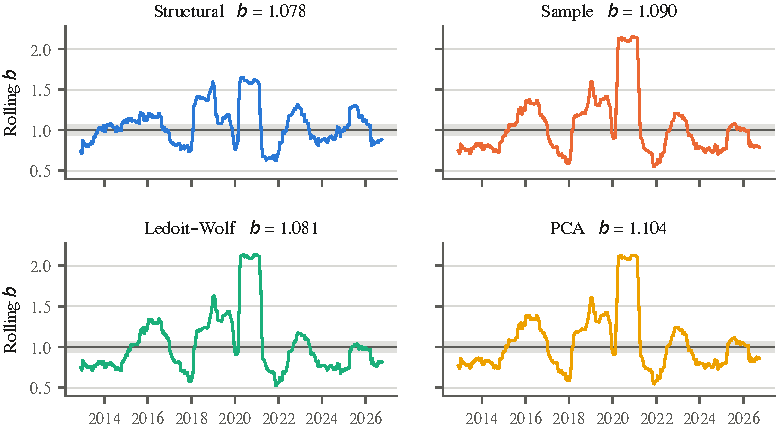
\includegraphics[width=0.94\linewidth]{figures/bias.pdf}
\caption{Rolling bias statistic for the minimum-variance portfolio under each
covariance estimator, on a 52-week window, against the shaded
$1\pm\sqrt{2/T}$ band. The band is a full-sample reference reproduced for
orientation, not a pointwise test for this series: it is derived under
independence, while successive points here share fifty-one weeks of history and
the underlying returns are themselves serially correlated, so excursions are
considerably less surprising than its width suggests. Panel titles give the
full-sample figure. Separate
panels rather than one axis because the three non-structural estimators trace
nearly identical paths and would overplot: the similarity is the point and a
single axis would hide it. All four exceed two during 2020, meaning realised
risk ran at roughly twice the forecast, and all four spend extended periods
below the band as well, so the full-sample figures above one are not a uniform
understatement through time.}
\label{fig:bias}
\end{figure}

Understating risk is not a surprise in a minimum-variance portfolio and it has
a known mechanism. \citet{goldberg2022dispersion} show that excess dispersion
in the leading eigenvector of an estimated covariance matrix propagates through
quadratic optimisation into the risk forecasts of the portfolios it produces,
with the optimiser selecting precisely the directions in which the estimate is
most overconfident. All four of our estimators sit outside the band on the same
side, which is consistent with that account and is not evidence for it over any
other.

There is also a formal counterpart to the argument of this section.
\citet{goldberg2025eigenvector} construct covariance estimates tailored to the
constraints a portfolio will be optimised under, shrinking the leading
eigenvector toward a subspace determined by the constraint gradients. That the
right estimate depends on the constraint set is the same proposition this
section argues empirically from the other direction: when the constraint set is
tight enough, estimates that differ substantially in isolation stop differing
where it counts. Their result is the stronger one, being analytic, and a
replication study is not the place to extend it; we note the connection because
it suggests the finding here is a special case of something general rather than
a feature of this index.

The practical reading is that an optimiser of this kind should not be trusted
to forecast its own risk, whichever of these four matrices sits underneath it.
That conclusion is unchanged across the estimator choice, which is the same
message the realised volatilities deliver from the other direction.

\section{What the constraints buy}
\label{sec:constraints}
Pending.

\section{Is low volatility an anomaly here?}
\label{sec:anomaly}
The low-volatility effect has been documented for decades, from
\citet{haugen1991efficient} through \citet{ang2006crosssection} and
\citet{blitz2007volatility}, and two accounts compete for it. One is a
leverage-constraint story: investors who want more market exposure than they
can borrow to obtain bid up high-beta stocks instead, leaving low-beta stocks
cheap \citep{frazzini2014betting}. The other is a benchmarking story: managers
judged against a capitalisation-weighted index treat low-beta positions as
risky in the only sense that matters to them, which deters the arbitrage that
would close the gap \citep{baker2011benchmarks}. Both predict that
low-volatility portfolios earn more than their market risk justifies, and they
differ in why.

Neither question is what a replication study is equipped to settle. What it can
do is ask whether the portfolios it built, and the funds they track, show
returns a standard factor model does not already account for.
Table~\ref{tab:alpha} reports intercepts on the \citet{fama2015five} five
factors plus momentum, then the same regressions with the
betting-against-beta factor added. Standard errors are those of
\citet{newey1987simple}, at eight lags, because daily returns on a
semi-annually rebalanced book are serially correlated and ordinary errors would
overstate significance.

\begin{table}[tbp]
\caption{Six-factor alphas before and after the betting-against-beta factor.}
\label{tab:alpha}
\centering\small
\setlength{\tabcolsep}{5pt}
\begin{tabular}{lrrrrrr}
\toprule
Portfolio & $\alpha$ (\%) & $t$ & $\alpha$+BAB (\%) & $t$ & $\beta_{\rm BAB}$ & $t$\\
\midrule
USMV, the fund & -0.17 & -0.10 & -1.96 & -1.45 & 0.309 & 12.2\\
USMV replica, structural & -0.07 & -0.09 & -0.54 & -0.71 & 0.099 & 10.3\\
USMV replica, sample & 0.58 & 0.66 & 0.16 & 0.19 & 0.113 & 8.8\\
USMV replica, Ledoit--Wolf & 0.91 & 0.96 & 0.51 & 0.58 & 0.116 & 9.6\\
USMV replica, PCA & 0.98 & 1.09 & 0.56 & 0.68 & 0.109 & 8.7\\
USMV replica, beta exempt & 0.34 & 0.28 & -0.84 & -0.80 & 0.241 & 13.6\\
\addlinespace
SPLV, the fund & -1.19 & -0.56 & -3.35 & -1.95 & 0.472 & 14.0\\
SPLV replica & -0.48 & -0.24 & -2.50 & -1.51 & 0.448 & 14.0\\
\bottomrule
\end{tabular}
\notetext{Daily excess returns regressed on the Fama--French five factors plus momentum, then re-run with the betting-against-beta factor added. Annualised intercepts, with Newey--West standard errors at 8 lags. The two blocks end on different dates because the factor vintages do: the six-factor window runs 2011-05-06 to 2026-08-31 and the seven-factor window to 2026-07-31, so the columns are not a paired test on an identical sample. No intercept reaches significance at the five per cent level in either block, though the largest, the SPLV fund's own at $t=-1.95$, falls only just short at $p=0.051$ and would clear a ten per cent threshold. Every betting-against-beta loading is significant by a wide margin, which is why the paper reads the pattern as absorption rather than as an absence of exposure.}
\end{table}


No intercept in either block reaches significance at the five per cent level.
The nearest is the heuristic fund's own, at $t=-1.95$ and $p=0.051$ once
betting-against-beta is included, and it is negative. Every
betting-against-beta loading is significant by a wide margin, with $t$ between
8.7 and 14.0 across every portfolio tested, and adding the factor moves each
intercept downward: the heuristic fund's annualised alpha falls from $-1.19\%$
to $-3.35\%$, the optimised fund's from $-0.17\%$ to $-1.96\%$.

Read carefully, this says something narrower than "the low-volatility anomaly
is explained". It says that over 2011 to 2026, in daily US large-cap data,
these particular portfolios earned no return that the five Fama--French factors
plus momentum fail to account for, and that their exposure to a
betting-against-beta portfolio is large and precisely estimated. A loading is
not a mechanism. The result is consistent with the leverage-constraint account
and it does not distinguish that account from the benchmarking one, because
both predict exactly this exposure; separating them requires evidence on
investor behaviour and constraint bindingness that daily return regressions
cannot supply.

Two further boundaries. The regressions end earlier than the portfolio results
because the factor vintages do, at 2026-08-31 for the six-factor block and
2026-07-31 once betting-against-beta is included, so the two blocks are not a
paired test on an identical sample and the table says so. And an intercept that
is not statistically distinguishable from zero is not an intercept shown to be
zero; with fifteen years of daily data the standard errors here are small, but
the finding is an absence of detected alpha, not a demonstration of its
absence.

\section{Interpretation and limitations}
\label{sec:limits}
Pending.

\section{Conclusion}
\label{sec:conclusion}
A rank-and-weight index rule is recoverable from its published description. A
constrained-optimisation rule is recoverable only up to the parts of its
description that are written in a vocabulary the reader does not have. Our
replica of the heuristic index tracks its fund at 1.62\% annualised tracking
error; our replica of the optimised index tracks at 5.83\%, and 2.10 percentage
points of that gap turn on how one noun phrase in the constraint document is
read.

The usual explanation for the difference does not survive measurement. Four
covariance estimators, from a singular sample matrix to a structural factor
model, track the fund within 26 basis points of one another under one
specification, against 2.10 percentage points for the exemption reading; a
block bootstrap separates the two intervals cleanly and the ordering holds in
every resample. That is what prior work reports for constrained portfolios
generally, and the reason is also known: binding constraints act as shrinkage,
so a tightly constrained feasible set leaves estimator differences nowhere to
express themselves. Our contribution on that point is confirmation in a
specific published constraint set, not discovery. What is new here is the
comparison of magnitudes, and the observation that the larger of the two
quantities is a reading of a document rather than a property of an estimator.

What the constraints deliver is not lower realised risk, which over this sample
they conspicuously fail to deliver, but control over where risk accumulates.
The sector band binds at every review examined; without it, the heuristic
accumulates an underweight to one industry that grows monotonically past forty
per cent. Both designs are concentrated, in different dimensions, and only one
of them concentrates by stated rule. Neither index shows a six-factor alpha
significant at the five per cent level, and betting-against-beta loadings
between 8.7 and 14.0 absorb what intercept there is, which is consistent with
the leverage-constraint account and does not distinguish it from the
benchmarking one.

The practical implication is narrow enough to state exactly. For anyone
replicating a constrained index from public data, effort spent resolving what
the methodology document actually specifies is worth more than effort spent
improving the covariance estimate, by a factor of about eight in this case. The broader implication, which this evidence motivates rather than
establishes, is that an index methodology stated in terms of a proprietary
factor model is not fully reproducible by construction, and that the gap this
creates is measurable and worth measuring.


\section*{Funding}
The author received no external funding for this work.

\section*{Disclosure statement}
The author declares no competing financial interests.

\section*{Data availability statement}
Every dataset behind the results is free to obtain and none is redistributed
here. Prices and corporate actions come from Yahoo Finance, fundamentals and
industry codes from the SEC's EDGAR XBRL interfaces, factor returns from the
Fama/French Data Library and AQR's public betting-against-beta series, and
point-in-time index membership from a public repository whose commit hash the
acquisition script records. The index methodology documents and the journal
articles cited are copyrighted and are not included; the source register in
the accompanying repository gives each one's identifier, retrieval location and
access date. One document, the S\&P 500 Low Volatility Index methodology,
refused the request from the run environment and was not retrieved; the single
parameter that depended on it is flagged in Section~\ref{sec:limits}.

\section*{Code availability}
The full pipeline, its tests and the frozen result tables behind every figure
and table in this paper are available from the author on reasonable request.

\section*{Declaration of generative AI use}
During the preparation of this work, the author used Claude in order to write
and run analysis code, revise and restructure the manuscript, check literature
and prepare the \LaTeX{} source. After using this tool/service, the author
reviewed and edited the content as needed and takes full responsibility for the
content of the published article.


\begingroup
\small
\setlength{\bibsep}{4pt}
% APA author-date reference list, rendered manually rather than through a .bst
% file. biber is unavailable in the build environment, apalike is not APA 7, and
% a hand-rendered thebibliography compiles wherever Overleaf puts it. natbib's
% authoryear mode takes the in-text form from the bracketed label.
%
% One deliberate departure from APA 7: the bracketed label supplies both the
% narrative and the parenthetical citation, so works with two authors read
% "Ledoit and Wolf (2003)" narratively and "(Ledoit and Wolf, 2003)" in
% parentheses, where APA would use an ampersand in the second. Labels are set
% for the narrative form because the text uses it predominantly. Reference-list
% entries themselves follow APA 7 exactly, ampersand included.
%
% Metadata mirrors references/references.bib, where every DOI was checked
% against Crossref. Do not edit an entry here without editing that file.
\begin{thebibliography}{99}

\bibitem[Alonso and Nusinzon(2020)]{alonso2020devil}
Alonso, N., \& Nusinzon, O. (2020). The devil is in the details: The risks
often ignored in low-volatility investing. \textit{The Journal of Portfolio
Management}, \textit{46}(7), 58--70.
\url{https://doi.org/10.3905/jpm.2020.1.163}

\bibitem[Ang et~al.(2006)]{ang2006crosssection}
Ang, A., Hodrick, R. J., Xing, Y., \& Zhang, X. (2006). The cross-section of
volatility and expected returns. \textit{The Journal of Finance},
\textit{61}(1), 259--299.
\url{https://doi.org/10.1111/j.1540-6261.2006.00836.x}

\bibitem[AQR Capital Management(n.d.)]{aqrbab}
AQR Capital Management. (n.d.). \textit{Betting against beta: Equity factors,
daily} [Data set]. Retrieved October 10, 2026, from
\url{https://www.aqr.com/Insights/Datasets/Betting-Against-Beta-Equity-Factors-Daily}

\bibitem[Bai and Ng(2002)]{bai2002determining}
Bai, J., \& Ng, S. (2002). Determining the number of factors in approximate
factor models. \textit{Econometrica}, \textit{70}(1), 191--221.
\url{https://doi.org/10.1111/1468-0262.00273}

\bibitem[Baker et~al.(2011)]{baker2011benchmarks}
Baker, M., Bradley, B., \& Wurgler, J. (2011). Benchmarks as limits to
arbitrage: Understanding the low-volatility anomaly. \textit{Financial Analysts
Journal}, \textit{67}(1), 40--54. \url{https://doi.org/10.2469/faj.v67.n1.4}

\bibitem[Blitz and van Vliet(2007)]{blitz2007volatility}
Blitz, D. C., \& van Vliet, P. (2007). The volatility effect. \textit{The
Journal of Portfolio Management}, \textit{34}(1), 102--113.
\url{https://doi.org/10.3905/jpm.2007.698039}

\bibitem[Blume(1971)]{blume1971assessment}
Blume, M. E. (1971). On the assessment of risk. \textit{The Journal of
Finance}, \textit{26}(1), 1--10.
\url{https://doi.org/10.1111/j.1540-6261.1971.tb00584.x}

\bibitem[Briner and Connor(2008)]{briner2008howmuch}
Briner, B., \& Connor, G. (2008). How much structure is best? A comparison of
market model, factor model and unstructured equity covariance matrices.
\textit{The Journal of Risk}, \textit{10}(4), 3--30.
\url{https://doi.org/10.21314/JOR.2008.180}

\bibitem[Clarke et~al.(2006)]{clarke2006minimum}
Clarke, R. G., de Silva, H., \& Thorley, S. (2006). Minimum-variance portfolios
in the U.S. equity market. \textit{The Journal of Portfolio Management},
\textit{33}(1), 10--24. \url{https://doi.org/10.3905/jpm.2006.661366}

\bibitem[DeMiguel et~al.(2009)]{demiguel2009optimal}
DeMiguel, V., Garlappi, L., \& Uppal, R. (2009). Optimal versus naive
diversification: How inefficient is the 1/N portfolio strategy? \textit{The
Review of Financial Studies}, \textit{22}(5), 1915--1953.
\url{https://doi.org/10.1093/rfs/hhm075}

\bibitem[Dom et~al.(2025)]{dom2025beyond}
Dom, M. S., Howard, C., Jansen, M., \& Lohre, H. (2025). Beyond GMV: The
relevance of covariance matrix estimation for risk-based portfolio
construction. \textit{Quantitative Finance}, \textit{25}(3), 403--419.
\url{https://doi.org/10.1080/14697688.2025.2468268}

\bibitem[Fama and French(2015)]{fama2015five}
Fama, E. F., \& French, K. R. (2015). A five-factor asset pricing model.
\textit{Journal of Financial Economics}, \textit{116}(1), 1--22.
\url{https://doi.org/10.1016/j.jfineco.2014.10.010}

\bibitem[Frazzini and Pedersen(2014)]{frazzini2014betting}
Frazzini, A., \& Pedersen, L. H. (2014). Betting against beta. \textit{Journal
of Financial Economics}, \textit{111}(1), 1--25.
\url{https://doi.org/10.1016/j.jfineco.2013.10.005}

\bibitem[French(n.d.)]{frenchdatalibrary}
French, K. R. (n.d.). \textit{Fama/French data library} [Data set]. Tuck School
of Business, Dartmouth College. Retrieved October 10, 2026, from
\url{https://mba.tuck.dartmouth.edu/pages/faculty/ken.french/data_library.html}

\bibitem[Goldberg et~al.(2022)]{goldberg2022dispersion}
Goldberg, L. R., Papanicolaou, A., \& Shkolnik, A. (2022). The dispersion bias.
\textit{SIAM Journal on Financial Mathematics}, \textit{13}(2), 521--550.
\url{https://doi.org/10.1137/21M144058X}

\bibitem[Haugen and Baker(1991)]{haugen1991efficient}
Haugen, R. A., \& Baker, N. L. (1991). The efficient market inefficiency of
capitalization-weighted stock portfolios. \textit{The Journal of Portfolio
Management}, \textit{17}(3), 35--40.
\url{https://doi.org/10.3905/jpm.1991.409335}

\bibitem[Invesco Exchange-Traded Fund Trust II(2024)]{invesco2024splv497k}
Invesco Exchange-Traded Fund Trust II. (2024). \textit{Invesco S\&P 500 Low
Volatility ETF summary prospectus} (Form 497K). U.S. Securities and Exchange
Commission.
\url{https://www.sec.gov/Archives/edgar/data/1378872/000119312524282757/d861761d497k.htm}

\bibitem[iShares Trust(2011)]{ishares2011usmv497k}
iShares Trust. (2011). \textit{iShares MSCI USA Minimum Volatility Index Fund
summary prospectus} (Form 497K). U.S. Securities and Exchange Commission.
\url{https://www.sec.gov/Archives/edgar/data/1100663/000119312511266729/d240179d497k.htm}

\bibitem[Jagannathan and Ma(2003)]{jagannathan2003risk}
Jagannathan, R., \& Ma, T. (2003). Risk reduction in large portfolios: Why
imposing the wrong constraints helps. \textit{The Journal of Finance},
\textit{58}(4), 1651--1683. \url{https://doi.org/10.1111/1540-6261.00580}

\bibitem[Ledoit and Wolf(2003)]{ledoit2003improved}
Ledoit, O., \& Wolf, M. (2003). Improved estimation of the covariance matrix of
stock returns with an application to portfolio selection. \textit{Journal of
Empirical Finance}, \textit{10}(5), 603--621.
\url{https://doi.org/10.1016/S0927-5398(03)00007-0}

\bibitem[Ledoit and Wolf(2004)]{ledoit2004honey}
Ledoit, O., \& Wolf, M. (2004). Honey, I shrunk the sample covariance matrix.
\textit{The Journal of Portfolio Management}, \textit{30}(4), 110--119.
\url{https://doi.org/10.3905/jpm.2004.110}

\bibitem[Markowitz(1952)]{markowitz1952portfolio}
Markowitz, H. (1952). Portfolio selection. \textit{The Journal of Finance},
\textit{7}(1), 77--91.
\url{https://doi.org/10.1111/j.1540-6261.1952.tb01525.x}

\bibitem[MSCI Inc.(2012)]{msci2012minvol}
MSCI Inc. (2012). \textit{MSCI minimum volatility indices methodology}.
Retrieved October 10, 2026, from
\url{https://www.msci.com/eqb/methodology/meth_docs/MSCI_Minimum_Volatility_Methodology_Jan12.pdf}

\bibitem[MSCI Inc.(2025)]{msci2025minvoladvanced}
MSCI Inc. (2025). \textit{MSCI minimum volatility advanced indexes
methodology}. Retrieved October 10, 2026, from
\url{https://www.msci.com/indexes/documents/methodology/3_MSCI_Minimum_Volatility_Advanced_Indexes_Methodology_20250203.pdf}

\bibitem[Newey and West(1987)]{newey1987simple}
Newey, W. K., \& West, K. D. (1987). A simple, positive semi-definite,
heteroskedasticity and autocorrelation consistent covariance matrix.
\textit{Econometrica}, \textit{55}(3), 703--708.
\url{https://doi.org/10.2307/1913610}

\bibitem[S\&P Dow Jones Indices(n.d.)]{spdji_lowvol_methodology}
S\&P Dow Jones Indices. (n.d.). \textit{S\&P 500 Low Volatility Index
methodology}.
\url{https://www.spglobal.com/spdji/en/documents/methodologies/methodology-sp-low-volatility-indices.pdf}

\bibitem[U.S. Securities and Exchange Commission(n.d.)]{secedgarapi}
U.S. Securities and Exchange Commission. (n.d.). \textit{EDGAR application
programming interfaces}. Retrieved October 10, 2026, from
\url{https://www.sec.gov/search-filings/edgar-application-programming-interfaces}

\end{thebibliography}

\endgroup

\appendix
\section{Identifying the market factor}
\label{app:identification}
Pending.

\section{The relaxation ladder as implemented}
\label{app:ladder}
The ladder below is transcribed from the provider's published infeasibility
procedure \citep{msci2012minvol}. Rung 0 is the published constraint set. The
solver attempts each rung in order and stops at the first that yields a
feasible book; if rung 12 fails, the review produces no trade and the previous
weights are carried forward unchanged.

\begin{table}[tbp]
\caption{The thirteen rungs, in the order attempted.}
\label{tab:ladder}
\centering\small
\setlength{\tabcolsep}{6pt}
\begin{tabular}{rrrrrl}
\toprule
Rung & Turnover & Min.\ holding & Weight cap & Sector band & What gave way\\
\midrule
 0 & 10\% & 5.0 bp & 1.5\% & 5.0\% & nothing; published set\\
\addlinespace
 1 & 15\% & 5.0 bp & 1.5\% & 5.0\% & turnover\\
 2 & 20\% & 5.0 bp & 1.5\% & 5.0\% & turnover\\
 3 & 25\% & 5.0 bp & 1.5\% & 5.0\% & turnover\\
 4 & 30\% & 5.0 bp & 1.5\% & 5.0\% & turnover\\
\addlinespace
 5 & 30\% & 4.0 bp & 1.5\% & 5.0\% & minimum holding\\
 6 & 30\% & 3.0 bp & 1.5\% & 5.0\% & minimum holding\\
 7 & 30\% & 2.0 bp & 1.5\% & 5.0\% & minimum holding\\
 8 & 30\% & 1.0 bp & 1.5\% & 5.0\% & minimum holding\\
\addlinespace
 9 & 30\% & 1.0 bp & 3.0\% & 5.0\% & weight cap\\
10 & 30\% & 1.0 bp & 3.0\% & 7.5\% & weight cap and sector\\
11 & 30\% & 1.0 bp & 5.0\% & 5.0\% & weight cap\\
12 & 30\% & 1.0 bp & 5.0\% & 7.5\% & weight cap and sector\\
\bottomrule
\end{tabular}
\notetext{The style band is 0.25 standard deviations at every rung, including
the last. It is the one bound the published procedure never relaxes, so a book
produced at any rung remains within 0.25 standard deviations of the parent on
every constrained style. Two features of this ordering would be easy to get
wrong by intuition: turnover is exhausted entirely before the minimum holding
is touched, and the weight cap and sector band move together rather than
separately. Across the 29 reviews in this study the ladder was needed between
two and seven times depending on the covariance estimator, and in nearly every
case a turnover rung sufficed; rung 12 was reached twice, once under the sample
estimator and once under the beta-exempt variant, and both of those reviews
produced no trade.}
\end{table}

\section{Parameters and their provenance}
\label{app:parameters}
Pending.


\end{document}
